\subsection{Endogeneity}%
\label{sub:endogeneity}

As discussed in Section~\ref{sub:estimation}, one concern one might have about
our results in Section~\ref{sec:results} is reverse causality:
transferring money into savings accounts might change the distribution of spend
categories and thus change entropy. As noted previously, this is not a major
concern because of the way we calculate savings and spend profiles: savings are
calculated as the sum of inflows into savings accounts, while spend profiles
are based on the classification of spend transactions in current accounts, and
transfers from current to savings accounts are labelled as such and not treated
as spend transactions.

However, because transaction labelling is imperfect, it is possible that some
transfers are misclassified as spends and included in the calculation of
entropy scores. One way to deal with this is to lag entropy scores by one
period. Table~\ref{tab:main_lag} presents results similar to the main
results in the main text, but using entropy lagged by one year-month period as
the independent variable of interest. We can see that the results are very
similar to thos presented above.

\def\yvars{has_inflows}
\foreach \y in \yvars {
    \begin{landscape}
    \begin{table}[ht]
    \centering\scriptsize
    \caption{Effect of lagged entropy on P(savings transactions)}
    \label{tab:main_lag}
    \input{\tabdir/reg_\y_lag.tex}
    \tabnote{.95\textwidth}{Results from estimating Equation~\ref{equ:model}. The
        dependent variable in all columns is a dummy variable indicating whether a
        user made at least one transaction into any of their savings accounts in a
    given period. Entropy variables are lagged by one period. \regtabinfo}
    \end{table}
    \end{landscape}
}

\subsection{Further results by financial resilience}%
\label{sub:results_by_financial_resilience}

The Tables below show results presented in
Section~\ref{sub:effect_of_financial_resilience} for alternative entropy
variables. 

\def\evars{entropy_tag, entropy_merchant}
\foreach \e in \evars {
    \input{\tabdir/reg_has_inflows_\e_z_inc_quint.tex}
    \input{\tabdir/reg_has_inflows_\e_sz_inc_quint.tex}
    \input{\tabdir/reg_has_inflows_\e_z_inc_var_quint.tex}
    \input{\tabdir/reg_has_inflows_\e_sz_inc_var_quint.tex}
}


\section{Scarcity}%
\label{sec:scarcity}

The economic literature on scarcity documents that our minds tend to focus on
what is scarce and neglect what is not, concentrating our mental resources
where they are most needed but impeding decision-making in other domains,
possibly leading to impaired and short-sighted decision
making\citep{shah2012some, mullainathan2013scarcity, haushofer2014psychology}.
For instance, \citet{mani2013poverty} find that low-income shoppers in New
Jersey perform worse on cognitive tasks when first promoted to think about
their financial situation while the same prompts had no effect for wealthier
shoppers, and sugarcane farmers in India perform worse on similar cognitive
tasks shortly before the annual harvest (when money is scarce) than shortly
thereafter (when money is plentiful). A prediction of this theory is that
people with low levels of savings find it hard to make sound spending decisions
as thir account balance dwindles, because their minds are increasingly captured
by financial worries. If high entropy spending behaviour captures life stress,
we would thus think that it is individuals with lowerer levels of incomes, who
have less mental bandwith to deal with said stress, that are most effected.

The results below show results similar to those presented in
Table~\ref{tab:reg_has_inflows_main} above, but separately for unsmoothed and
smoothed income and separately for each income quintile and income variation
quintile, respectively.


\begin{table}[htbp]
   \centering
   \tiny
   \begin{threeparttable}[b]
      \caption{\label{tab:reg_has_inflows_entropy_tag_spend_z_inc_quint} Effect of entropy on P(has savings) by income quintile}
      \begin{tabular}{lccccc}
         \tabularnewline \midrule \midrule
         Model:             & (1)             & (2)             & (3)            & (4)            & (5)\\  
         Income quintile:   & 1               & 2               & 3              & 4              & 5 \\   
         \midrule
         \emph{Variables}\\
         Entropy (48 cats)  & 0.033$^{***}$   & 0.019$^{***}$   & 0.017$^{***}$  & 0.016$^{***}$  & 0.018$^{***}$\\   
                            & [0.028; 0.039]  & [0.013; 0.025]  & [0.011; 0.023] & [0.010; 0.022] & [0.012; 0.025]\\   
         Month spend        & 0.010$^{***}$   & 0.007$^{***}$   & 0.008$^{***}$  & 0.007$^{***}$  & 0.006$^{***}$\\   
                            & [0.009; 0.011]  & [0.006; 0.008]  & [0.006; 0.009] & [0.006; 0.008] & [0.005; 0.007]\\   
         Month income       & 0.015$^{***}$   & 0.010$^{***}$   & 0.012$^{***}$  & 0.013$^{***}$  & 0.008$^{***}$\\   
                            & [0.012; 0.019]  & [0.004; 0.017]  & [0.005; 0.019] & [0.008; 0.019] & [0.007; 0.010]\\   
         Income variability & -0.000          & 0.001           & 0.002$^{***}$  & 0.001$^{**}$   & -0.000\\   
                            & [-0.001; 0.001] & [-0.000; 0.002] & [0.001; 0.004] & [0.000; 0.002] & [-0.001; 0.001]\\   
         \midrule
         \emph{Fixed-effects}\\
         User               & Yes             & Yes             & Yes            & Yes            & Yes\\  
         Year-month         & Yes             & Yes             & Yes            & Yes            & Yes\\  
         \midrule
         \emph{Fit statistics}\\
         Observations       & 223,462         & 215,151         & 208,417        & 201,319        & 195,378\\  
         R$^2$              & 0.59138         & 0.58949         & 0.58354        & 0.58212        & 0.57162\\  
         Within R$^2$       & 0.00535         & 0.00180         & 0.00211        & 0.00191        & 0.00271\\  
         \midrule \midrule
         \multicolumn{6}{l}{\emph{Clustered (User) co-variance matrix, 95\% confidence intervals in brackets}}\\
         \multicolumn{6}{l}{\emph{Signif. Codes: ***: 0.01, **: 0.05, *: 0.1}}\\
      \end{tabular}
   \end{threeparttable}
\end{table}




\begin{table}[htbp]
   \centering
   \tiny
   \begin{threeparttable}[b]
      \caption{\label{tab:reg_has_inflows_entropy_tag_spend_sz_inc_quint} Effect of entropy on P(has savings) by income quintile}
      \begin{tabular}{lccccc}
         \tabularnewline \midrule \midrule
         Model:                    & (1)              & (2)              & (3)              & (4)              & (5)\\  
         Income quintile:          & 1                & 2                & 3                & 4                & 5 \\   
         \midrule
         \emph{Variables}\\
         Entropy (48 cats, smooth) & -0.026$^{***}$   & -0.020$^{***}$   & -0.017$^{***}$   & -0.015$^{***}$   & -0.017$^{***}$\\   
                                   & [-0.030; -0.023] & [-0.024; -0.016] & [-0.021; -0.013] & [-0.019; -0.011] & [-0.021; -0.012]\\   
         Month spend               & 0.009$^{***}$    & 0.006$^{***}$    & 0.007$^{***}$    & 0.007$^{***}$    & 0.006$^{***}$\\   
                                   & [0.008; 0.011]   & [0.005; 0.007]   & [0.006; 0.008]   & [0.005; 0.008]   & [0.005; 0.007]\\   
         Month income              & 0.015$^{***}$    & 0.010$^{***}$    & 0.012$^{***}$    & 0.013$^{***}$    & 0.008$^{***}$\\   
                                   & [0.012; 0.019]   & [0.004; 0.017]   & [0.004; 0.019]   & [0.007; 0.019]   & [0.007; 0.010]\\   
         Income variability        & -0.000           & 0.001            & 0.002$^{***}$    & 0.001$^{**}$     & -0.000\\   
                                   & [-0.001; 0.001]  & [-0.000; 0.002]  & [0.001; 0.004]   & [0.000; 0.002]   & [-0.001; 0.001]\\   
         \midrule
         \emph{Fixed-effects}\\
         User                      & Yes              & Yes              & Yes              & Yes              & Yes\\  
         Year-month                & Yes              & Yes              & Yes              & Yes              & Yes\\  
         \midrule
         \emph{Fit statistics}\\
         Observations              & 223,462          & 215,151          & 208,417          & 201,319          & 195,378\\  
         R$^2$                     & 0.59152          & 0.58970          & 0.58369          & 0.58223          & 0.57175\\  
         Within R$^2$              & 0.00570          & 0.00230          & 0.00246          & 0.00216          & 0.00302\\  
         \midrule \midrule
         \multicolumn{6}{l}{\emph{Clustered (User) co-variance matrix, 95\% confidence intervals in brackets}}\\
         \multicolumn{6}{l}{\emph{Signif. Codes: ***: 0.01, **: 0.05, *: 0.1}}\\
      \end{tabular}
   \end{threeparttable}
\end{table}





\begin{table}[htbp]
   \centering
   \tiny
   \begin{threeparttable}[b]
      \caption{\label{tab:reg_has_inflows_entropy_tag_spend_z_inc_var_quint} Effect of entropy on P(has savings) by income variability quintile}
      \begin{tabular}{lccccc}
         \tabularnewline \midrule \midrule
         Model:                       & (1)             & (2)            & (3)             & (4)             & (5)\\  
         Income variability quintile: & 1               & 2              & 3               & 4               & 5 \\   
         \midrule
         \emph{Variables}\\
         Entropy (48 cats)            & 0.020$^{***}$   & 0.014$^{***}$  & 0.022$^{***}$   & 0.028$^{***}$   & 0.021$^{***}$\\   
                                      & [0.014; 0.026]  & [0.008; 0.020] & [0.016; 0.028]  & [0.022; 0.034]  & [0.015; 0.027]\\   
         Month spend                  & 0.008$^{***}$   & 0.008$^{***}$  & 0.007$^{***}$   & 0.007$^{***}$   & 0.007$^{***}$\\   
                                      & [0.007; 0.009]  & [0.007; 0.009] & [0.006; 0.008]  & [0.006; 0.008]  & [0.006; 0.008]\\   
         Month income                 & 0.014$^{***}$   & 0.010$^{***}$  & 0.011$^{***}$   & 0.010$^{***}$   & 0.010$^{***}$\\   
                                      & [0.011; 0.017]  & [0.008; 0.012] & [0.010; 0.013]  & [0.009; 0.012]  & [0.009; 0.011]\\   
         Has income in month          & 0.092$^{***}$   & 0.076$^{***}$  & 0.064$^{***}$   & 0.055$^{***}$   & 0.067$^{***}$\\   
                                      & [0.073; 0.111]  & [0.056; 0.095] & [0.047; 0.081]  & [0.040; 0.070]  & [0.053; 0.081]\\   
         Income variability           & -0.001          & 0.006$^{**}$   & -0.000          & 0.000           & -0.004$^{**}$\\   
                                      & [-0.003; 0.001] & [0.001; 0.011] & [-0.004; 0.003] & [-0.001; 0.002] & [-0.007; -0.001]\\   
         \midrule
         \emph{Fixed-effects}\\
         User                         & Yes             & Yes            & Yes             & Yes             & Yes\\  
         Year-month                   & Yes             & Yes            & Yes             & Yes             & Yes\\  
         \midrule
         \emph{Fit statistics}\\
         Observations                 & 223,462         & 215,151        & 208,417         & 201,319         & 195,378\\  
         R$^2$                        & 0.61166         & 0.59951        & 0.59062         & 0.59379         & 0.63519\\  
         Within R$^2$                 & 0.00558         & 0.00398        & 0.00484         & 0.00579         & 0.00781\\  
         \midrule \midrule
         \multicolumn{6}{l}{\emph{Clustered (User) co-variance matrix, 95\% confidence intervals in brackets}}\\
         \multicolumn{6}{l}{\emph{Signif. Codes: ***: 0.01, **: 0.05, *: 0.1}}\\
      \end{tabular}
   \end{threeparttable}
\end{table}




\begin{table}[htbp]
   \centering
   \tiny
   \begin{threeparttable}[b]
      \caption{\label{tab:reg_has_inflows_entropy_tag_spend_sz_inc_var_quint} Effect of entropy on P(has savings) by income variability quintile}
      \begin{tabular}{lccccc}
         \tabularnewline \midrule \midrule
         Model:                       & (1)              & (2)              & (3)              & (4)              & (5)\\  
         Income variability quintile: & 1                & 2                & 3                & 4                & 5 \\   
         \midrule
         \emph{Variables}\\
         Entropy (48 cats, smooth)    & -0.019$^{***}$   & -0.020$^{***}$   & -0.017$^{***}$   & -0.022$^{***}$   & -0.024$^{***}$\\   
                                      & [-0.024; -0.015] & [-0.024; -0.016] & [-0.021; -0.013] & [-0.026; -0.018] & [-0.028; -0.019]\\   
         Month spend                  & 0.007$^{***}$    & 0.007$^{***}$    & 0.006$^{***}$    & 0.006$^{***}$    & 0.006$^{***}$\\   
                                      & [0.006; 0.008]   & [0.006; 0.008]   & [0.005; 0.008]   & [0.005; 0.007]   & [0.005; 0.007]\\   
         Month income                 & 0.014$^{***}$    & 0.010$^{***}$    & 0.011$^{***}$    & 0.010$^{***}$    & 0.010$^{***}$\\   
                                      & [0.011; 0.017]   & [0.008; 0.012]   & [0.009; 0.013]   & [0.009; 0.012]   & [0.009; 0.011]\\   
         Has income in month          & 0.093$^{***}$    & 0.075$^{***}$    & 0.064$^{***}$    & 0.056$^{***}$    & 0.066$^{***}$\\   
                                      & [0.074; 0.112]   & [0.055; 0.094]   & [0.047; 0.081]   & [0.040; 0.071]   & [0.052; 0.081]\\   
         Income variability           & -0.001           & 0.005$^{**}$     & -0.000           & 0.000            & -0.004$^{**}$\\   
                                      & [-0.003; 0.001]  & [0.001; 0.010]   & [-0.004; 0.003]  & [-0.001; 0.002]  & [-0.006; -0.001]\\   
         \midrule
         \emph{Fixed-effects}\\
         User                         & Yes              & Yes              & Yes              & Yes              & Yes\\  
         Year-month                   & Yes              & Yes              & Yes              & Yes              & Yes\\  
         \midrule
         \emph{Fit statistics}\\
         Observations                 & 223,462          & 215,151          & 208,417          & 201,319          & 195,378\\  
         R$^2$                        & 0.61181          & 0.59979          & 0.59070          & 0.59394          & 0.63550\\  
         Within R$^2$                 & 0.00597          & 0.00466          & 0.00502          & 0.00614          & 0.00864\\  
         \midrule \midrule
         \multicolumn{6}{l}{\emph{Clustered (User) co-variance matrix, 95\% confidence intervals in brackets}}\\
         \multicolumn{6}{l}{\emph{Signif. Codes: ***: 0.01, **: 0.05, *: 0.1}}\\
      \end{tabular}
   \end{threeparttable}
\end{table}





\section{Effect of entropy on overdraft fees}%
\label{sub:effect_of_entropy_on_overdraft_fees}

\begin{itemize}

    \item Table~\ref{tab:reg_entropy_odfees} replicates results from
        \citet{muggleton2020evidence} Tables S20 (Columns 1 and 2) and Table
        S40 (columns 3 and 4).

    \item Similar to their results, higher entropy is positively related to
        negative financial outcomes.

    \item Yet, contrary to their findings, the effect becomes stronger in the
        presence of fixed effects.

    \item Also, in contrast to above findings, using non-smoothed entropy
        doesn't reverse the effect but strengthen it.

    \item Differences to \citet{muggleton2020evidence} could be due to a number
        of factors: we use a different dataset, a different and self-selected sample of people
        that is skewed towards younger and wealthier individuals, as well as a
        longer panel.

\end{itemize}


\begin{table}[htbp]
   \centering
   \caption{\label{tab:reg_entropy_odfees} Effect of entropy on overdraft fees}
   \begin{scriptsize}
      \begin{tabular}{lcccc}
         \tabularnewline\midrule\midrule
         Dependent Variable: & \multicolumn{4}{c}{has\_od\_fees}\\
         Model:                      & (1)                     & (2)                     & (3)            & (4)\\
         \midrule \emph{Variables} &   &   &   &  \\
         Entropy (tag-based, smooth) & 0.0040$^{**}$           &                         & 0.0052$^{*}$   &   \\
                                     & (0.0018)                &                         & (0.0027)       &   \\
         Entropy (tag-based)         &                         & 0.0745$^{***}$          &                & 0.0318$^{***}$\\
                                     &                         & (0.0029)                &                & (0.0044)\\
         Spend communication         & 0.6974$^{***}$          & 0.5952$^{***}$          & 0.1294$^{***}$ & 0.1025$^{***}$\\
                                     & (0.0256)                & (0.0258)                & (0.0385)       & (0.0384)\\
         Spend finance               & 0.0256$^{***}$          & 0.0192$^{***}$          & 0.0124$^{***}$ & 0.0110$^{***}$\\
                                     & (0.0028)                & (0.0028)                & (0.0037)       & (0.0037)\\
         Spend hobbies               & 0.0040                  & -0.1075$^{***}$         & 0.0411         & 0.0106\\
                                     & (0.0283)                & (0.0284)                & (0.0263)       & (0.0265)\\
         Spend household             & -0.0011                 & 0.0018                  & 0.0027         & 0.0033\\
                                     & (0.0016)                & (0.0016)                & (0.0021)       & (0.0021)\\
         Spend other                 & 0.0188$^{***}$          & 0.0072$^{*}$            & -0.0053        & -0.0091$^{**}$\\
                                     & (0.0040)                & (0.0040)                & (0.0040)       & (0.0040)\\
         Spend motor                 & 0.1373$^{***}$          & 0.0441$^{***}$          & 0.0326         & 0.0068\\
                                     & (0.0154)                & (0.0157)                & (0.0208)       & (0.0208)\\
         Spend retail                & 0.0109                  & -0.0124$^{*}$           & 0.0018         & -0.0063\\
                                     & (0.0073)                & (0.0074)                & (0.0068)       & (0.0070)\\
         Spend services              & -0.0073$^{**}$          & 0.0085$^{**}$           & -0.0054        & -0.0026\\
                                     & (0.0036)                & (0.0035)                & (0.0039)       & (0.0038)\\
         Spend travel                & -0.0329$^{***}$         & -0.0449$^{***}$         & -0.0041        & -0.0078$^{**}$\\
                                     & (0.0049)                & (0.0049)                & (0.0036)       & (0.0036)\\
         Female                      & 0.0429$^{***}$          & 0.0367$^{***}$          & -0.3720        & -0.3891\\
                                     & (0.0030)                & (0.0030)                & (47,268.6)     & (47,267.8)\\
         Age                         & -0.0026$^{***}$         & -0.0026$^{***}$         &                &   \\
                                     & (0.0001)                & (0.0001)                &                &   \\
         Year income                 & -0.0015$^{***}$         & -0.0015$^{***}$         & 0.0005$^{*}$   & 0.0005\\
                                     & ($9.26\times 10^{-5}$) & ($9.22\times 10^{-5}$) & (0.0003)       & (0.0003)\\
         (Intercept)                 & 0.2793$^{***}$          & 0.2746$^{***}$          &                &   \\
                                     & (0.0057)                & (0.0056)                &                &   \\
         \midrule \emph{Fixed-effects} &   &   &   &  \\
         User id                     &                         &                         & Yes            & Yes\\
         Calendar month              &                         &                         & Yes            & Yes\\
         \midrule \emph{Fit statistics} &   &   &   &  \\
         Observations                & 82,589                  & 82,589                  & 82,589         & 82,589\\
         R$^2$                       & 0.02522                 & 0.03275                 & 0.63492        & 0.63561\\
         Within R$^2$                &                         &                         & 0.00162        & 0.00352\\
         \midrule\midrule\multicolumn{5}{l}{\emph{Signif. Codes: ***: 0.01, **: 0.05, *: 0.1}}\\
      \end{tabular}
   \end{scriptsize}
\end{table}





\paragraph{Shopping-time based entropy}
\label{par:shopping_time_based_entropy}

We calculate entropy based on the probability of $(day of week, merchant)$
tuples, where we follow \citet{guidotti2015behavioral} and bin \textit{day of
week} into \textit{weekends} and \textit{weekday}, to reduce excessive
fluctuations. Because banks tend to process weekend transactions on Monday, as
shown in Figure~\ref{fig:spending}, we cannot distinguish transactions made on
Saturdays or Sundays from those made on Mondays, and thus classify all of them
as weekend transactions. We drop the about 25 percent of transactions for which
we cannot identify a merchant. The alternative would be leaving these
transactions in the sample and treating ``unknown merchant'' as a single
merchant. But for user-months for which the merchant is unknown for all
transactions, this would lead to an entropy score of 0, which is undesireable.

\paragraph{Grocery shop entropy}%
\label{par:grocery_shop_entropy}

We consider purchases at Tesco, Sainsbury's, Asda, Morrisons, Aldi, Co-op,
Lidl, Waitrose, Iceland, and Ocado, which have a combined market share of 96.5
percent.

\section{Savings patterns}%
\label{sec:savings_patterns}

survey examples
%https://www.mckinsey.com/capabilities/growth-marketing-and-sales/our-insights/how-us-consumers-are-feeling-shopping-and-spending-and-what-it-means-for-companies
%https://www.bls.gov/cex/

based on debit card data:
%https://www.barclayscorporate.com/insights/industry-expertise/uk-consumer-spending-report/
%https://www.ons.gov.uk/peoplepopulationandcommunity/personalandhouseholdfinances/expenditure/bulletins/familyspendingintheuk/april2019tomarch2020

% \begin{figure}[H]
%     \center \newcommand\width{\textwidth} \caption{Savings behaviour}
%     \label{fig:savings}
%     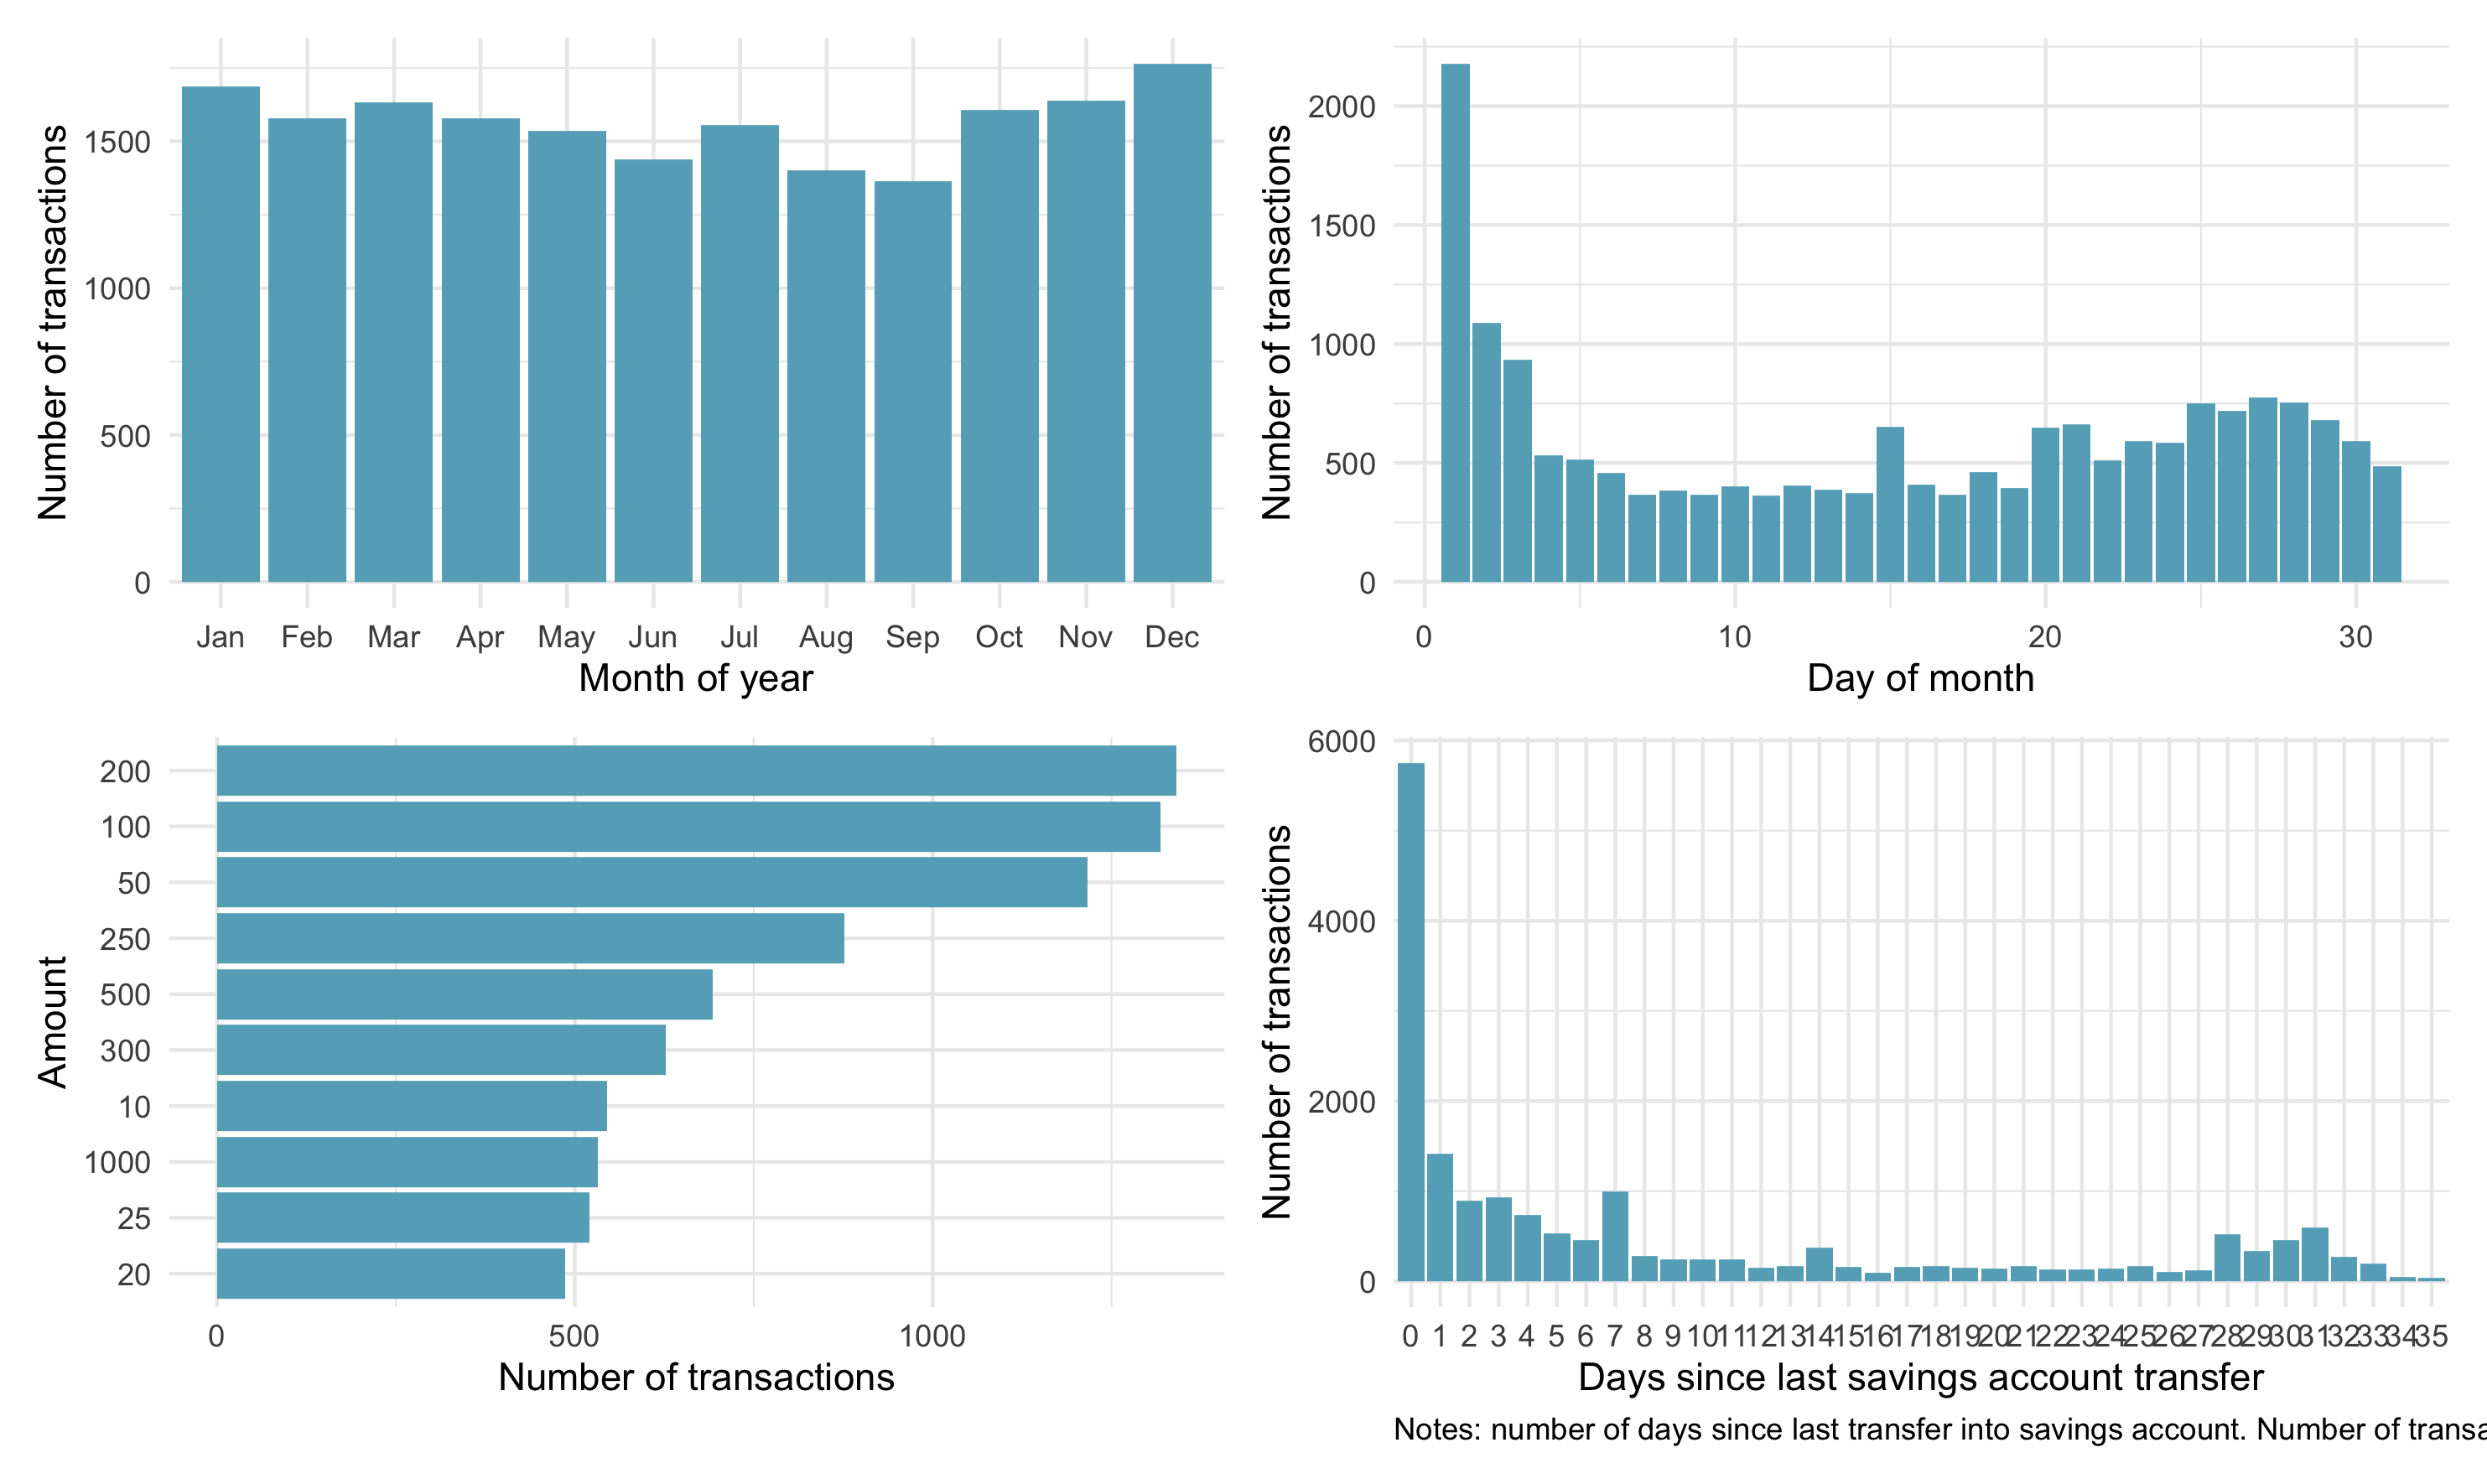
\includegraphics[width=\width]{\figdir/savings.png}
% \end{figure}

